\documentclass[12pt, a4paper]{article}
\usepackage{graphicx}
\usepackage{pgfplots}
\usepackage{mathtools}
\usepackage{fancyhdr}
\usepackage{multicol}
\usepackage{cancel}
\usepackage{geometry}
\usepackage{listings}
\usepackage{booktabs}
\usepackage{tabularx}
\usepackage{subfig}
\usepackage{hyperref}
\usepackage{float}
\usepackage{titlesec}
\usepackage{tikz, pgfplots}
\usepackage[utf8]{inputenc}
\usepackage[backend=biber,style=ieee]{biblatex}

% Requirement libs
\usetikzlibrary{positioning}

% Options
\nonstopmode % To make sure that you dont have to press input for each error
\geometry{top=1in, left = 1in, right = 1in, bottom=1.2in}
\pgfplotsset{compat=1.18}
\graphicspath{{./figures/}}
\setlength{\columnsep}{0.7cm}

% Metadata
\bibliography{./citations.bib}
\addbibresource{./citations.bib}
\author{Aris Podotas}
\date{today}

% Herlink setup
\hypersetup{
    colorlinks=true,
    linkcolor=blue,
    filecolor=magenta,
    urlcolor=cyan,
    pdftitle={MLICB Assignment 1},
    pdfpagemode=FullScreen,
}

% For the code blocks
\definecolor{codegreen}{rgb}{0.03,0.5,0.03}
\definecolor{codegray}{rgb}{0.5,0.5,0.5}
\definecolor{codepurple}{rgb}{0.58,0,0.82}
\definecolor{backcolour}{rgb}{0.95,0.95,0.95}

% Code block setup
\lstdefinestyle{mystyle}{
    backgroundcolor=\color{backcolour},
    commentstyle=\color{codegreen},
    keywordstyle=\color{magenta},
    numberstyle=\tiny\color{codegray},
    stringstyle=\color{codepurple},
    basicstyle=\ttfamily\footnotesize,
    breakatwhitespace=false,
    breaklines=true,
    captionpos=b,
    keepspaces=true,
    numbers=left,
    numbersep=5pt,
    showspaces=false,
    showstringspaces=false,
    showtabs=false,
    tabsize=4,
    escapeinside = {(*}{*)}
}
\lstset{style=mystyle}

% My custom headers and margins 
\pagestyle{fancy}
\setlength{\headheight}{44pt}
\setlength{\headsep}{18pt}
\lhead{\includegraphics[scale = 0.2]{./figures/bnw unit.png}}
\chead{\quad Data Science and Information Technologies Master’s
National and Kapodistrian University of Athens}
\rhead{}
\lfoot{}
\cfoot{\thepage}
\rfoot{}

% Start
\begin{document}

% Custom title page
\begin{titlepage}
    \centering
    {\huge \textbf{Assignment 2}\par}
    \vspace{0.5cm}
    {\Large \textbf{Name:} Aris Podotas\par}
    \vspace{0.5cm}
    {\large \textbf{University:} National and Kapodistrian University of Athens\par}
    \vspace{0.5cm}
    {\large \textbf{Program:} Data Science and Information Technologies\par}
    \vspace{0.5cm}
    {\large \textbf{Specialization:} Bioinformatics - Biomedical Data\par}
    \vspace{0.5cm}
    {\large \textbf{Lesson:} Machine Learning In Computational Biology\par}
    \vspace{0.5cm}
    {\large \textbf{Date:} May 2025\par}
    \tableofcontents
\end{titlepage}

\begin{multicols}{2}

    \section*{Abstract} \label{sec:abs}

    The task of properly classifying tumors into benign and malignant categories using machine learning has been a focal point of the $21^{st}$ century. Here we use the advances of machine learning as a field to try and propose methods of completing this classification in a non trivial way.
    \newline

    \section{Introduction} \label{sec:intro}

    In classification task like the one of categorizing tumors into benign and malignant categories, the trivial solution is to focus on the inequality of the two sets. Should a model always predict a benign tumor it would have a good accuracy over all instances due to the how frequent the benign tumors are over the malignant ones. For this reason this classification task remains prominent in the machine learning space. It is critical to develop reliable methods for doing this classification since domain knowledge takes years to attain and mistakes are critical and costly. Benign tumors can appear in all tissues through ones lifetime, at any points a multitude of factors may convert a benign tumor to a malignant one \cite{koten_transition_1991}, \cite{koten_difference_1993}.
    \newline

    Catching malignant tumors early can be crucial for the survival and cost of treatment for women with breast cancer and thus it is important to have apt methodology that can accurately distinguish between benign and malignant tumors \cite{din_breast_2022}. Machine learning models have been developed for calcifications of breast cancer tumors ranging from mammography, ultrasound, MRI, histology, and thermography \cite{radak_machine_2023}. Images of fine needle aspirates as in our data will contribute to the available methods of classification for this cause.
    \newline

    \section{Methods} \label{sec:methods}

    \subsection{Implementation} \label{subsec:impl}

    All results were created in the \textit{Python} programming language \cite{noauthor_3132_nodate}. Functionality from \href{https://github.com/ArisPodotas/Assignment-1-MLICB}{this repository} (last assignment) was also used in the analysis.
    \newline

    All source files will be available in \href{https://github.com/ArisPodotas/Assignment-2-MLICB/tree/master}{this repository}.
    \newline

    The approach of the implementation was of OOP (Object Oriented Programming) and all requirements are completed within two classes, a utility class (implemented \href{https://github.com/ArisPodotas/Assignment-2-MLICB/blob/master/src/utils.py}{here}) and a RNCV (Repeated Nested Cross Validation) class (implemented \href{https://github.com/ArisPodotas/Assignment-2-MLICB/blob/master/src/classes.py}{here}).
    \newline

    \subsection{Models} \label{subsec:models}

    Models:
    \newline

    \begin{enumerate} \label{enm:models}
        \item Logistic Regression
        \item Gaussian Naive Bayes
        \item Linear Discriminant Analysis
        \item Support Vector Classifier
        \item Random Forest Classifier
    \end{enumerate}

    Models were imported from the \textit{sklearn} \cite{noauthor_scikit-learn_nodate} library in \textit{Python} \cite{noauthor_3132_nodate}.
    \newline

    \subsection{Evaluation metrics} \label{subsec:metrics}

    The following evaluation metrics were chosen:
    \newline

    \begin{enumerate} \label{enm:metrics}
        \item balanced accuracy score 
        \item f1 score
        \item Hamming loss
        \item fbeta score
        \item Jaccard score
        \item Matthews corrcoef
        \item precision score
        \item recall score
    \end{enumerate}

    We will not be using the "Auc" metrics since our task is not fit for it. For the fbeta score we have used a beta of $2$ since we would like to give the negative and less represented class more weight.
    \newline

    \subsection{Confidences} \label{subsec:conf}

    \textit{Repeated nested K-fold cross validation} for $10$ folds, $5$ outer folds and $3$ inner folds were done for each model as per the requirements. Each individual evaluation of any model at any stage is calculated but only kept in memory momentarily, the results of each evaluation is seen only within the plots produced by the class. Individual evaluations from the inner folds outer folds and each loop are calculated and plotted in boxplots that try to capture the distribution space of each models evaluation rather than singular evaluation values.
    \newline

    \subsection{Figures} \label{subsec:figs}

    Figures were generated from the \textit{matplotlib} \cite{noauthor_matplotlib_nodate} library, all implementations are available at \href{https://github.com/ArisPodotas/Assignment-2-MLICB}{our source files}.
    \newline

    In all box plots the dotted green line denotes the mean value and the orange line denotes the median value.
    \newline

    \subsection{Missing data} \label{subsec:missing}

    Since missing data was found our strategy for the handling of such entries will be to replace the entry with the median value of the feature in questions. We will choose the median to be more resilient to outliers since we will see that the mean has been affected over the median.
    \newline

    \subsection{Classes} \label{subsec:class}

    A utility class (implemented \href{https://github.com/ArisPodotas/Assignment-2-MLICB/blob/master/src/utils.py}{here}) and a RNCV (Repeated Nested Cross Validation) class (implemented \href{https://github.com/ArisPodotas/Assignment-2-MLICB/blob/master/src/classes.py}{here}) were written according to the following diagram.
    \newline

\end{multicols}

    \begin{figure}[H]
        \begin{center}
            \includegraphics[width=0.95\textwidth]{figures/rcv.png}
        \end{center}
        \caption{Flow chart of class implementation}\label{fig:class outline}
    \end{figure}

\begin{multicols}{2}

    This figure was made in \href{https://excalidraw.com}{Excalidraw}. Only the main aspects of the class are written in the flow diagram since other implementation details are not part of the purpose of the class such as the "\_\_repr\_\_()" magic method.
    \newline

    The "RNCV" class has an attribute of a "Utility" class instance object and that is why these two have control flow from one into the other.
    \newline

    \subsection{Data transformations} \label{subsec:transforms}

    Most of our data is of continuous variables that need no interpolation of any sort considering there are fields for mean values standard errors and "worst cases". We will convert the diagnosis field to a binary values one where:
    \newline

    \begin{enumerate} \label{enm:casting}
        \item B $\rightarrow \; 0$
        \item M $\rightarrow \; 1$
    \end{enumerate}

    \subsection{Feature selection} \label{subsec:fselect}

    For the main requirements of the assignment a Principled Component Analysis was used (after the baseline models). We will require a 95\% explain of our data variance after the feature selection.
    \newline

    For further feature selections see \ref{subsec:bonus1}
    \newline

    \subsection{Hyper parameter optimization} \label{subsec:optuna}

    The optuna library \cite{noauthor_optuna_nodate} was used for all hyperparameter tuning (only in an instance after the baseline). All optimizations are in relation to the fbeta score since we would like to define the beta parameter of this metric to $2$ for a higher weight on the smaller positive class.
    \newline

    \section{Results} \label{sec:res}

    \subsection{Data Exploration} \label{subsec:expl}

\end{multicols}

    \begin{figure}[H]
        \begin{center}
            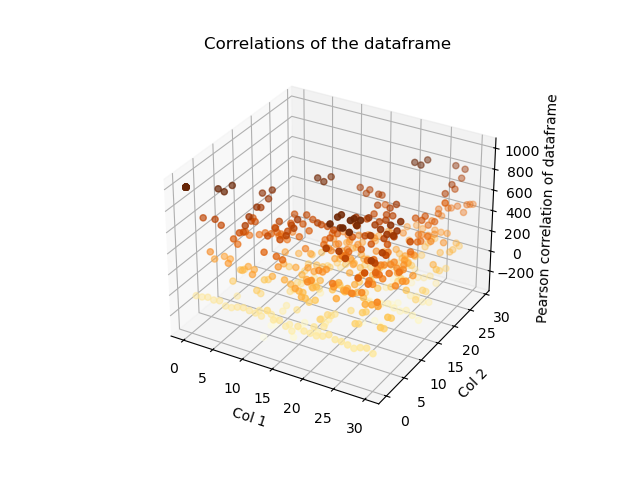
\includegraphics[width=0.95\textwidth]{figures/Correlations of the dataframe.png}
        \end{center}
        \caption{Pearson correlation of all feature pairs}\label{fig:corr}
    \end{figure}

\begin{multicols}{2}

    We can see that there is a lot of pruning to be done for features that are correlated in Figure~\ref{fig:corr}.
    \newline

\end{multicols}

    \begin{figure}[H]
        \begin{center}
            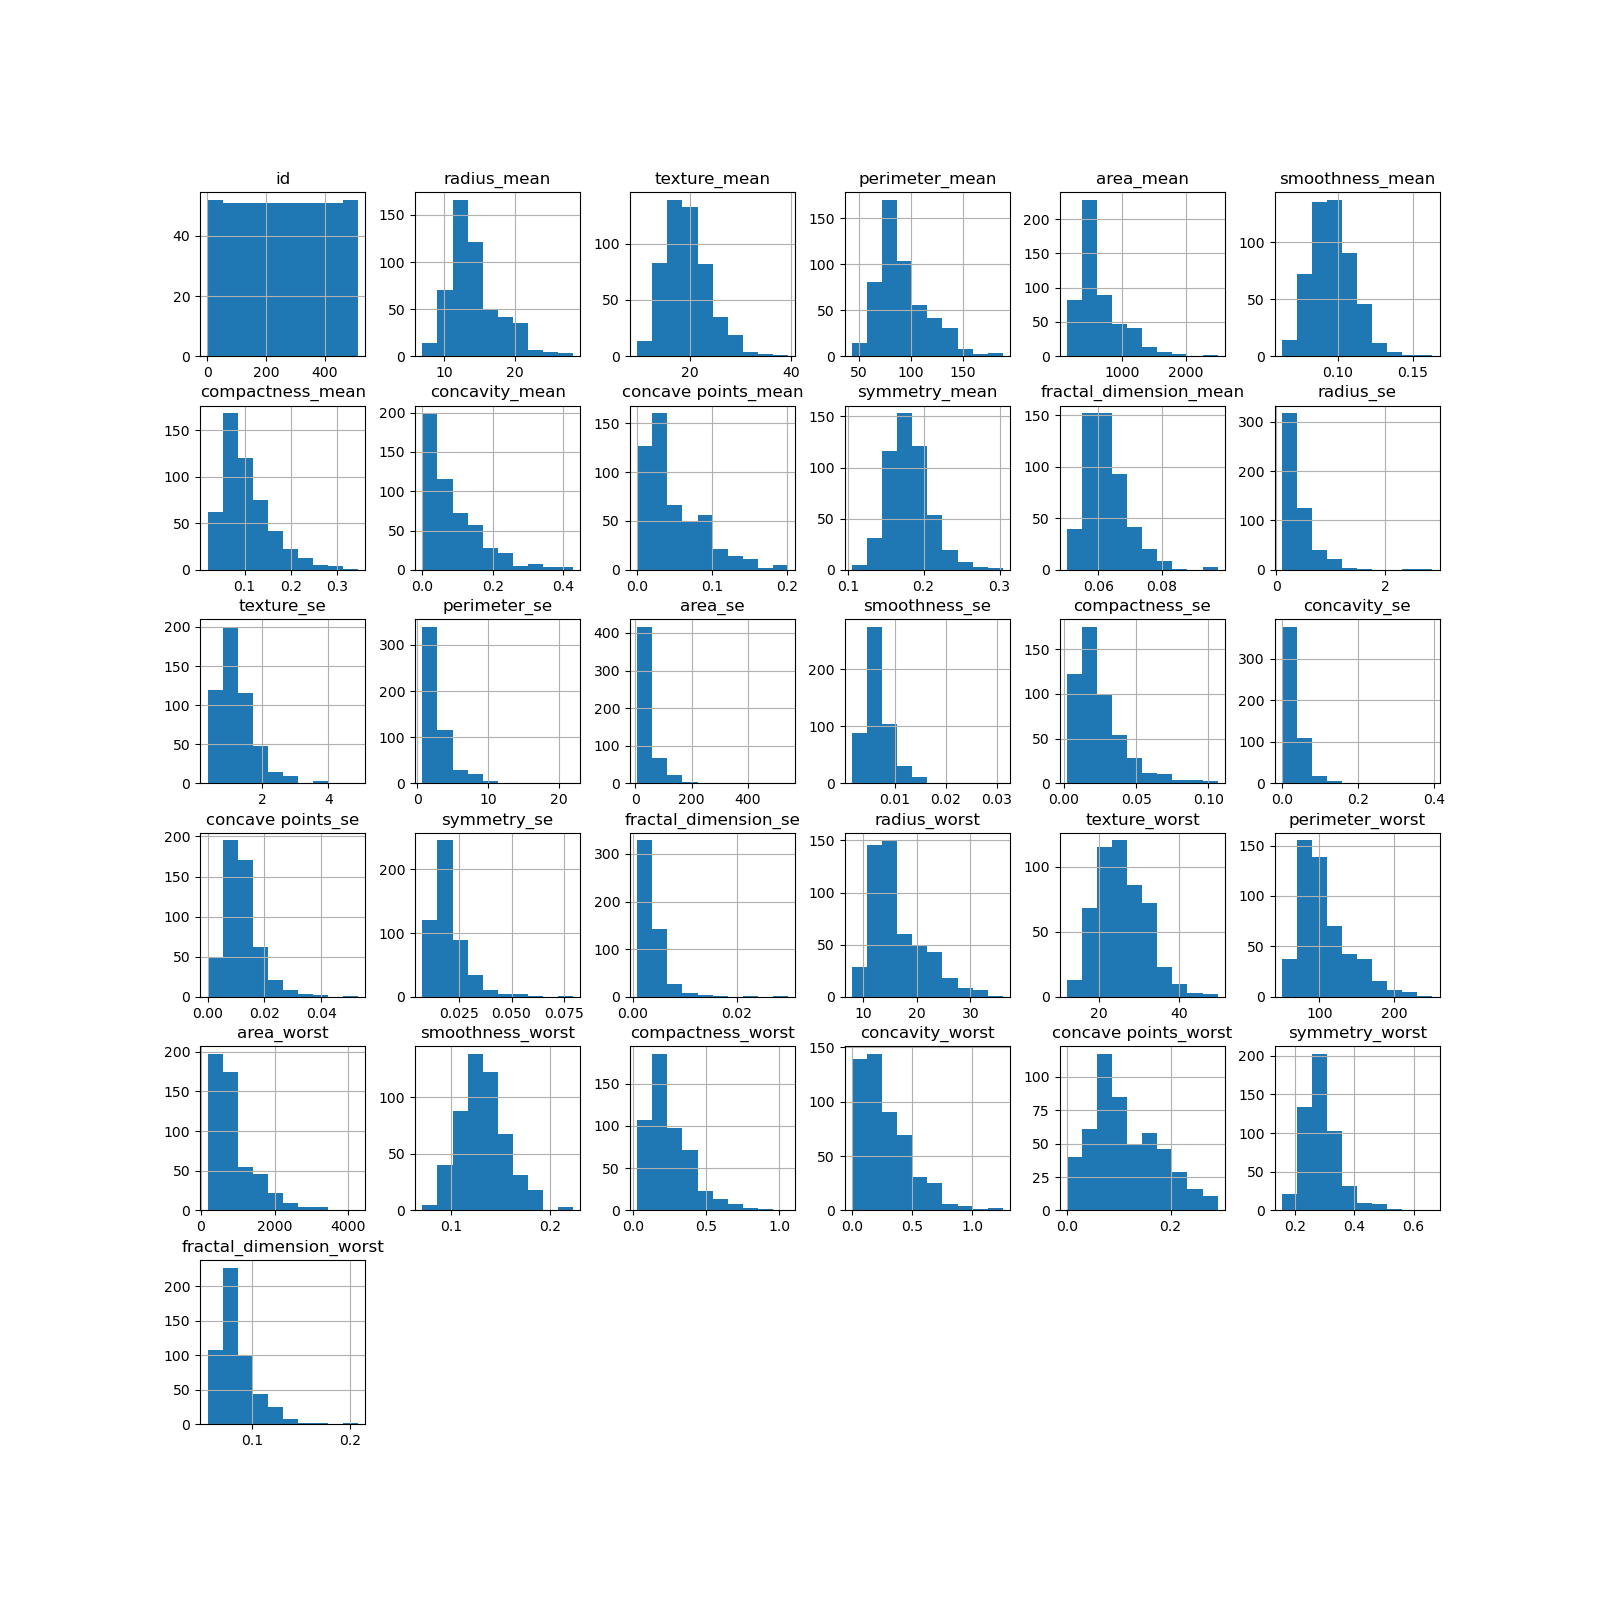
\includegraphics[width=0.95\textwidth]{figures/Data feature histograms.png}
        \end{center}
        \caption{Distribution of values for each feature}\label{fig:hists}
    \end{figure}

\begin{multicols}{2}

    We can make some sort of comment on the appearance of the central limit theorem in Figure~\ref{fig:hists} considering we get a Gaussian looking distribution \cite{kwak_central_2017} from taking the mean values of feature's distributions.
    \newline

\end{multicols}

\begin{figure}[H]
    \begin{center}
        
\includegraphics[width=0.95\textwidth]{figures/Explain of all principaled components.png}
    \end{center}
    \caption{Explain \% of all principal components}\label{fig:PCA search}
\end{figure}

    We can see that very few principled components will be needed for the 95\% variance explain we will require. Specifically we will see that only $2$ features reach this percentage (other than the labels).
    \newlinw

\begin{multicols}{2}

    Descriptive statistics were calculated for the initial data in the \href{https://github.com/ArisPodotas/Assignment-2-MLICB/blob/master/notebooks/Feeling%20the%20data.ipynb}{respective notebook} and then saved to \href{https://github.com/ArisPodotas/Assignment-2-MLICB/blob/master/data/statistics.csv}{this comma separated values file}.
    \newline

    \subsection{Baseline} \label{subsec:baseline}

    We are tasked with evaluating this data completely thus we need to identify data types and cast fields to values we can use. Our data was of continuous values variables for all fields but one, that was converted to a binary field as was mentioned in \ref{subsec:transforms}. Immediately after and with no feature selection or optimization the baseline model was made.
    \newline

    Evaluations of the Baseline:
    \newline

\end{multicols}

\begin{figure}[H]
    \begin{center}
        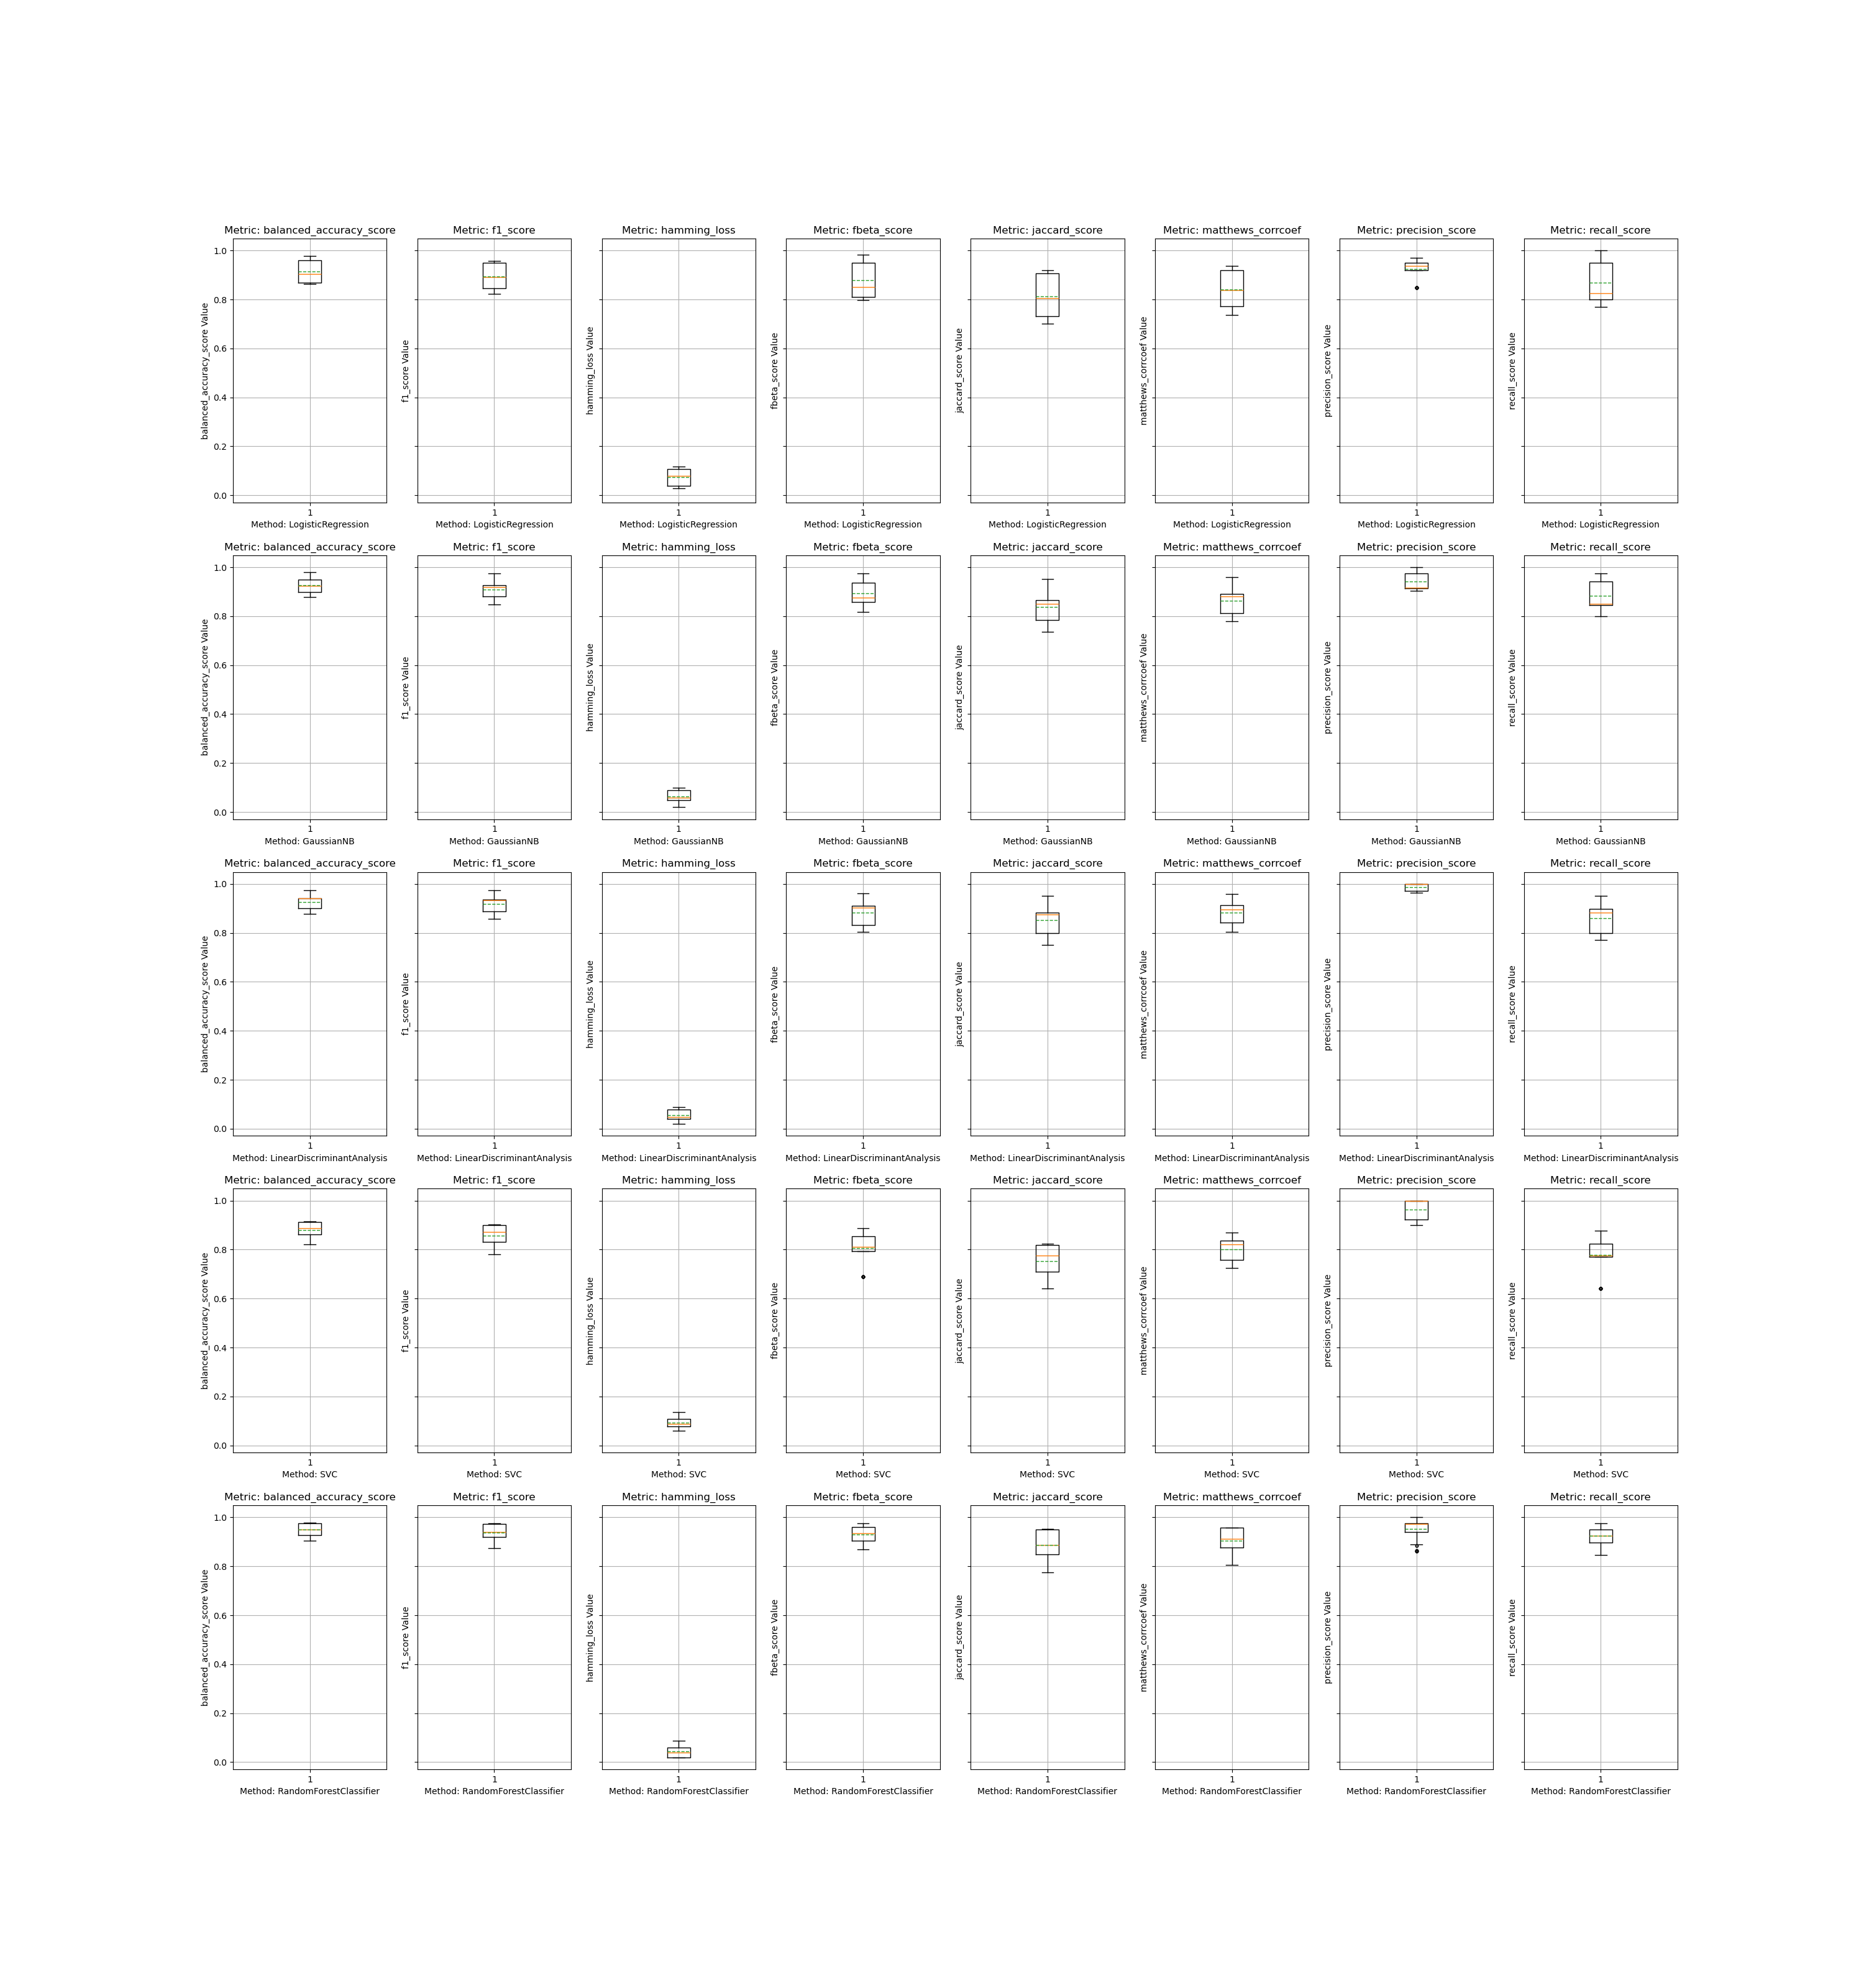
\includegraphics[width=0.95\textwidth]{figures/RNCV/Baseline/All loop outer folds boxplots.png}
        \caption{Final distributions of all loops of the baseline model}\label{fig:Baseline descriptive statistics}
    \end{center}
\end{figure}

\begin{multicols}{2}

    You can find the baseline model in \href{https://github.com/ArisPodotas/Assignment-2-MLICB/tree/master/models/Baseline}{in this folder}. As was said in \ref{subsec:optuna} one of the best descriptive statistics here is the fbeta score. It is easy for our models to simply always predict benign and get high metrics but the fbeta score is weighed toward the proper predictions of the malignant tumors.
    \newline

    \subsection{Feature selection} \label{subsec:fs}

\end{multicols}

\begin{figure}[H]
    \begin{center}
        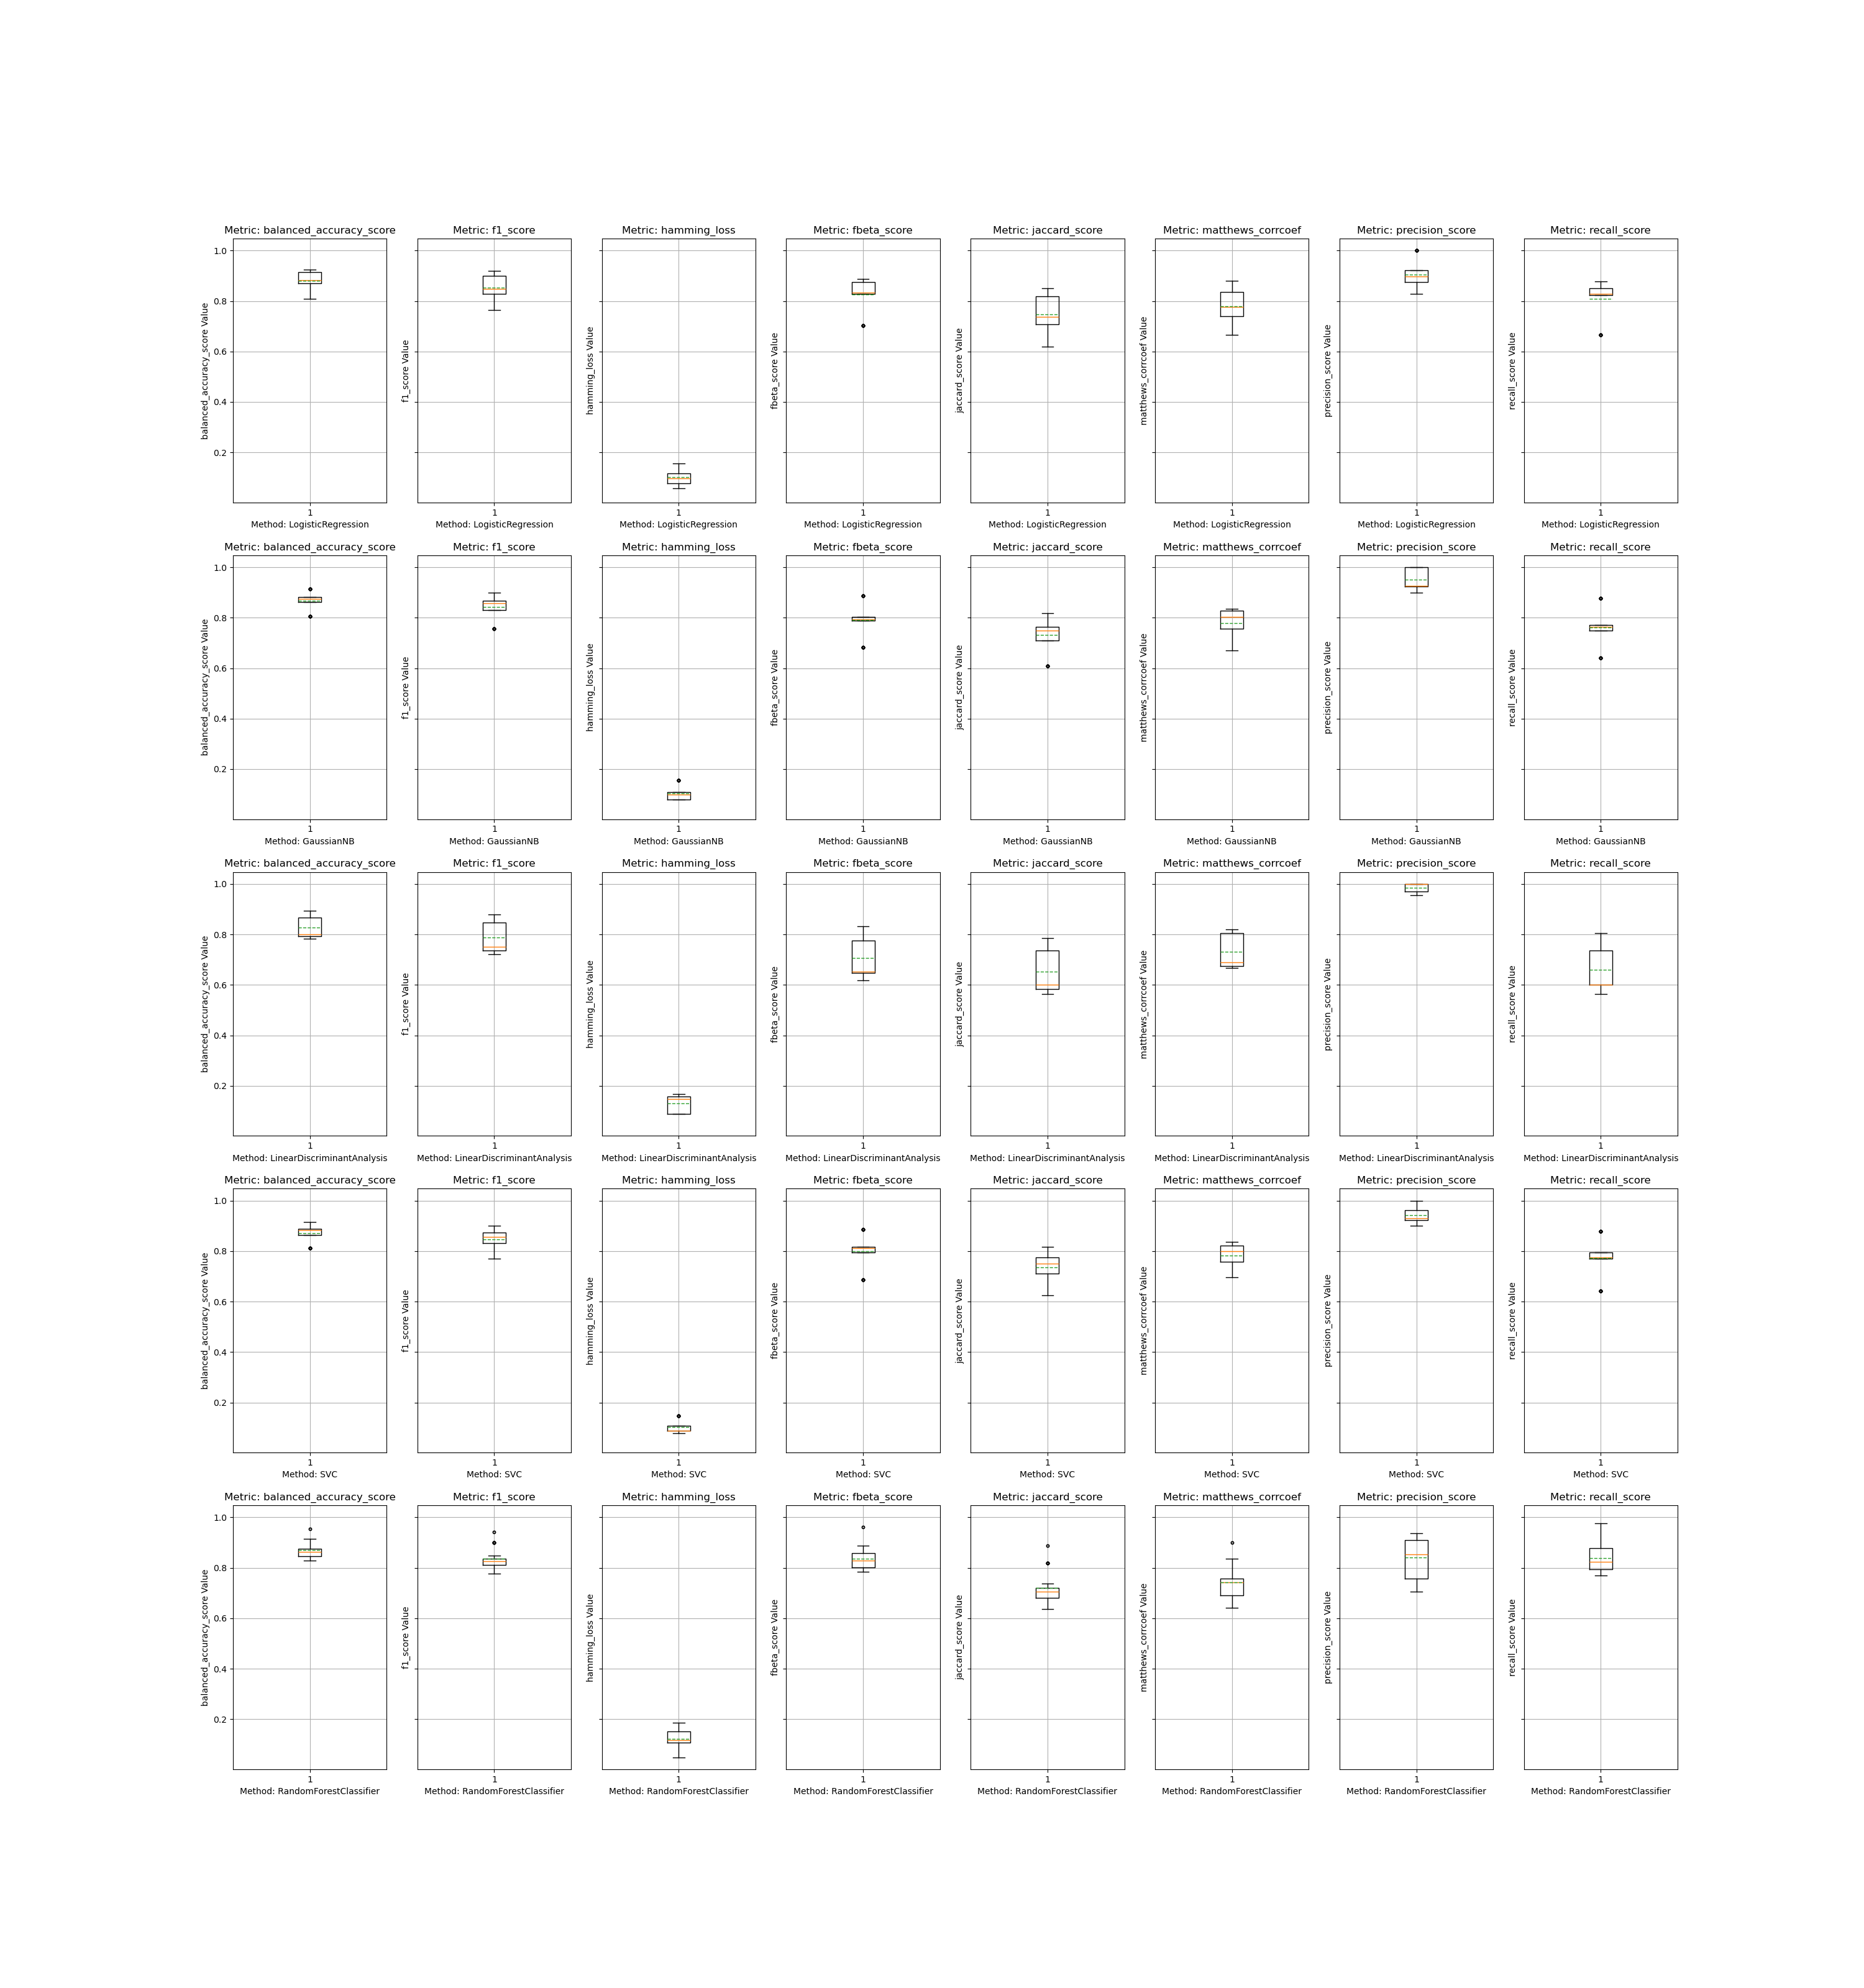
\includegraphics[width=0.95\textwidth]{figures/RNCV/FeatureSelection/All loop outer folds boxplots.png}
        \caption{Final distributions of all loops of the feature selected model}\label{fig:fs model desc}
    \end{center}
\end{figure}

\begin{multicols}{2}

    We notice that the metrics do not improve much since there is little space to improve from the Baseline~\ref{subsec:baseline}. Infact we expect that since we prune so many of our features to only remain with $2$ form the initial $31$ our metrics would decrease, here we see a resilience to this and a very good explanatory feature in our data.
    \newlin

    \subsection{Bonus 1} \label{subsec:bonus1}

    The previous feature selection method was a PCA, now we will try Select k best with a metric of $X^2$ and compare it to the previous feature selection however we will not take it into account for our winner model and the final conclusions to be fair.
    \newline

\end{multicols}

\begin{figure}[H]
    \begin{center}
        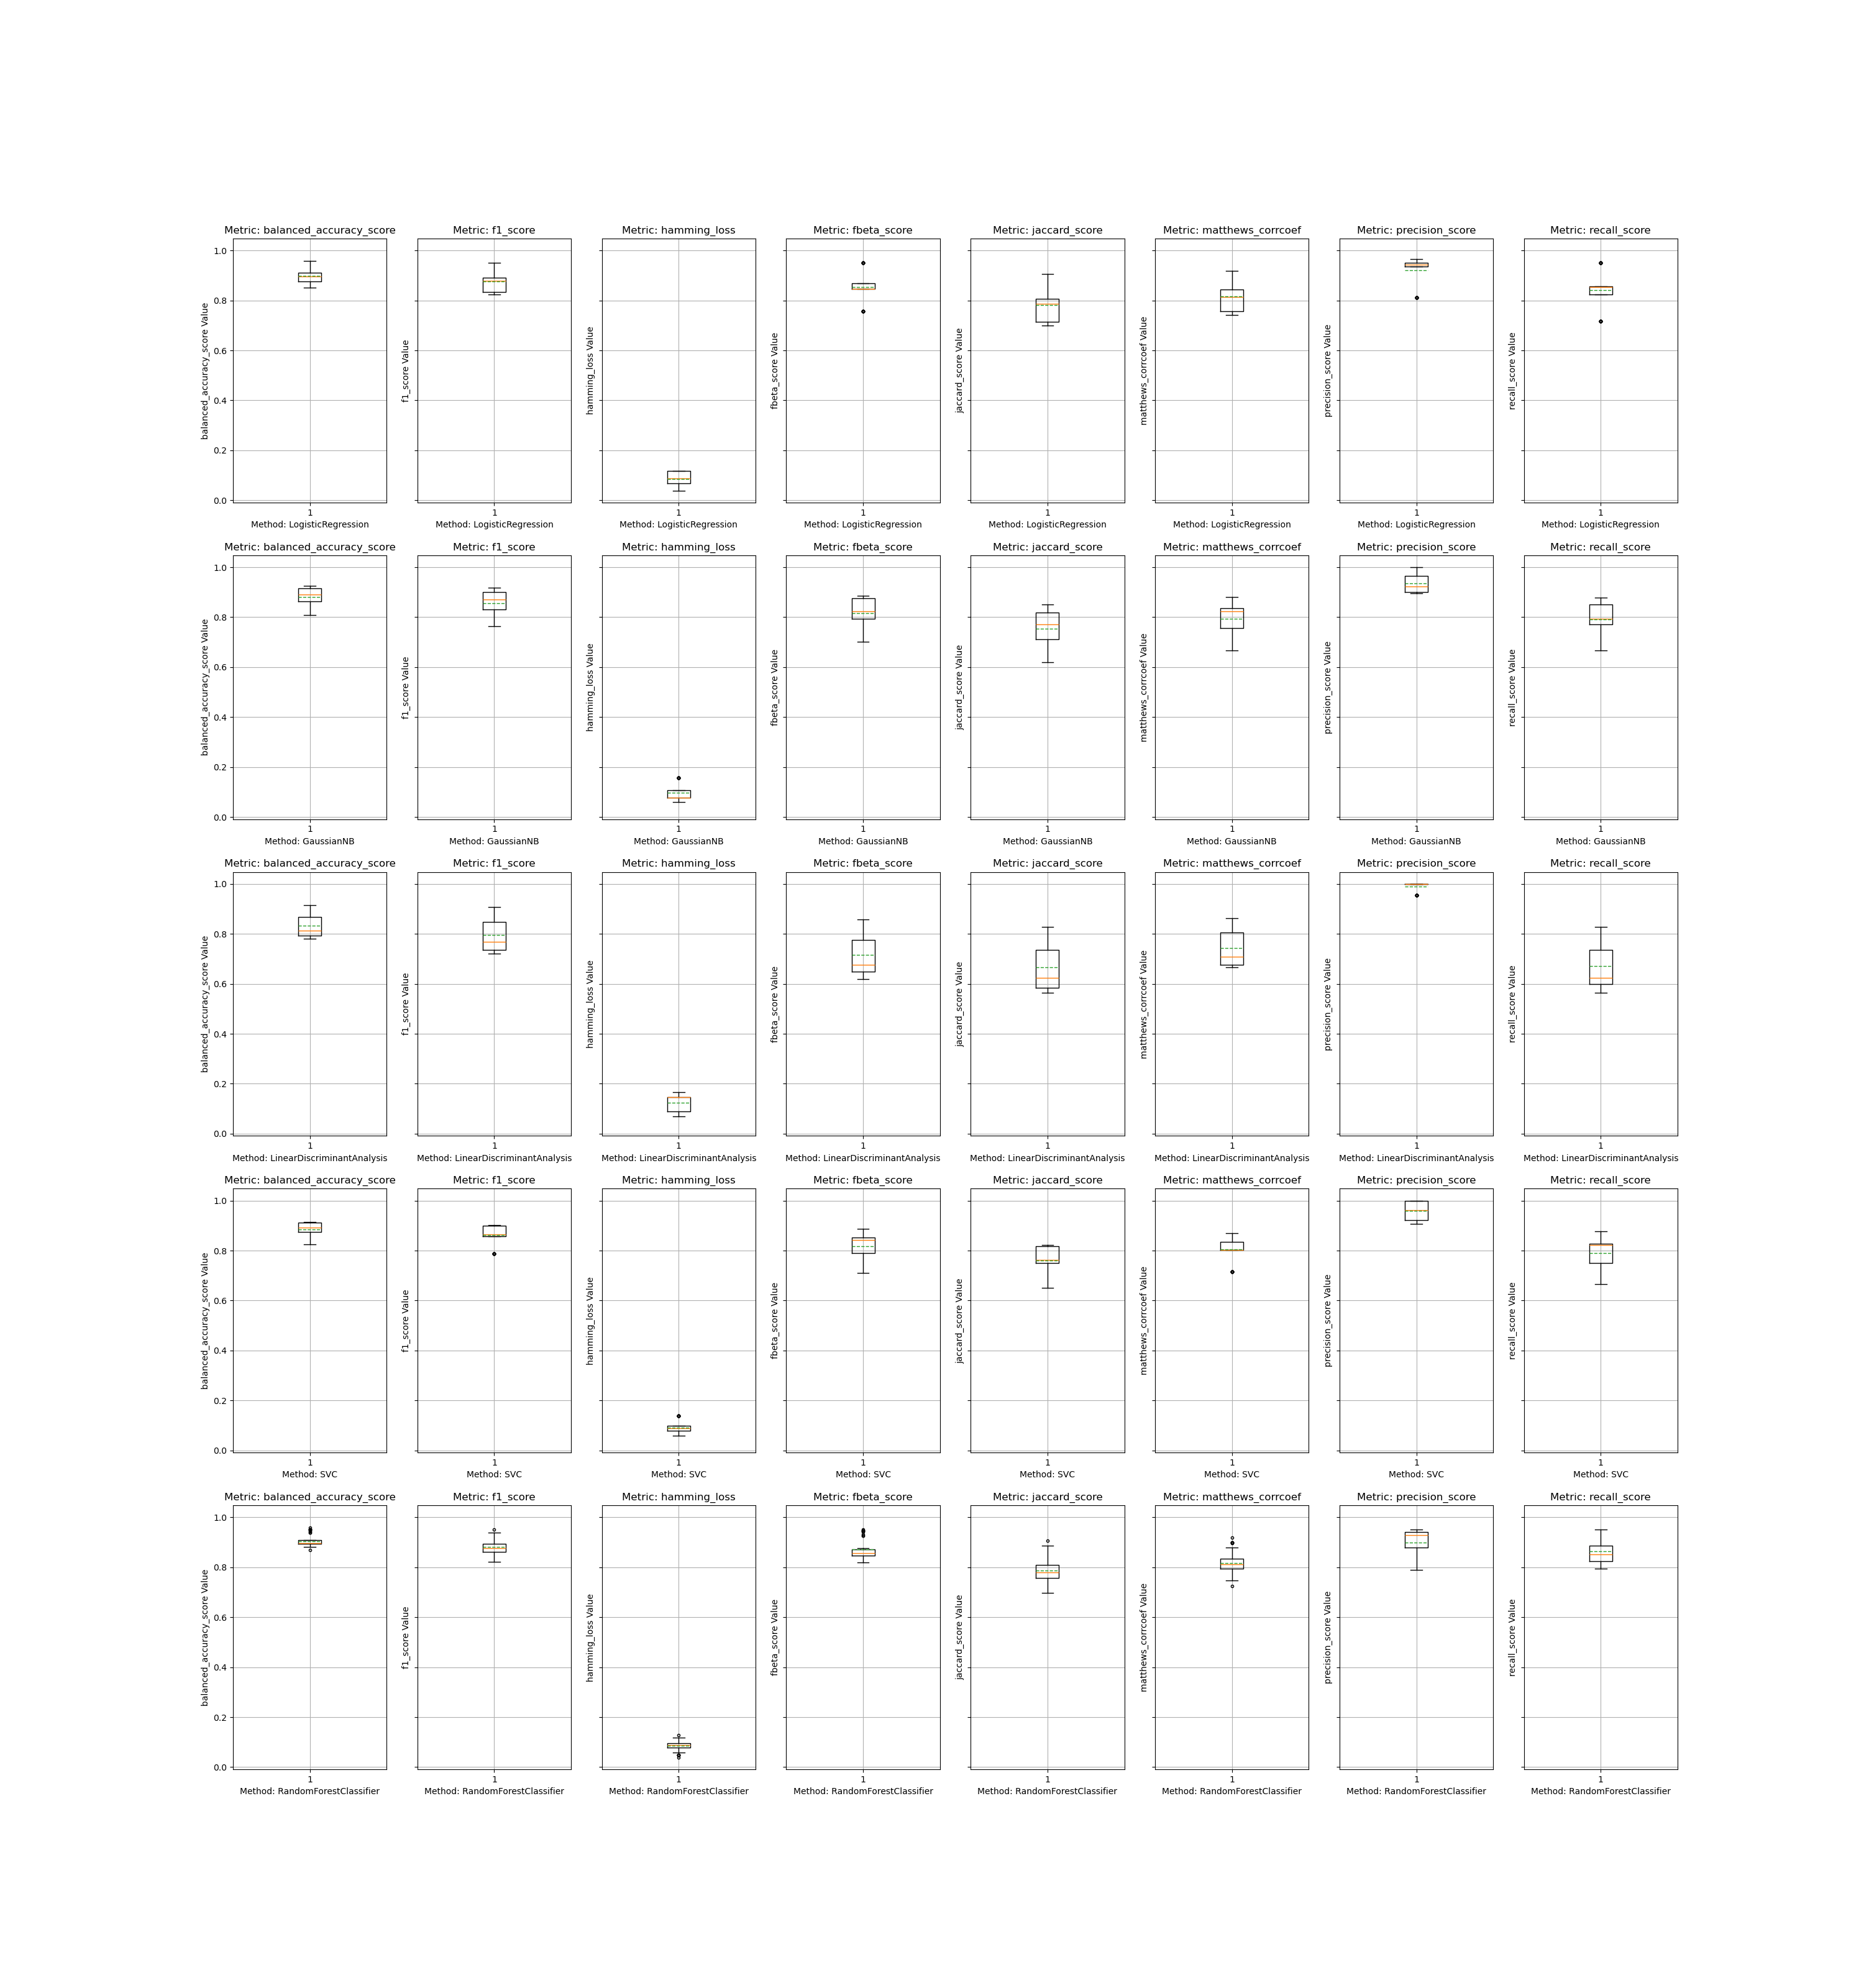
\includegraphics[width=0.95\textwidth]{figures/RNCV/Bonus/All loop outer folds boxplots.png}
        \caption{Final distributions of all loops of the feature selected model using $X^2$ Select k best}\label{fig:bonus}
    \end{center}
\end{figure}

\begin{figure}[H]
    \begin{center}
        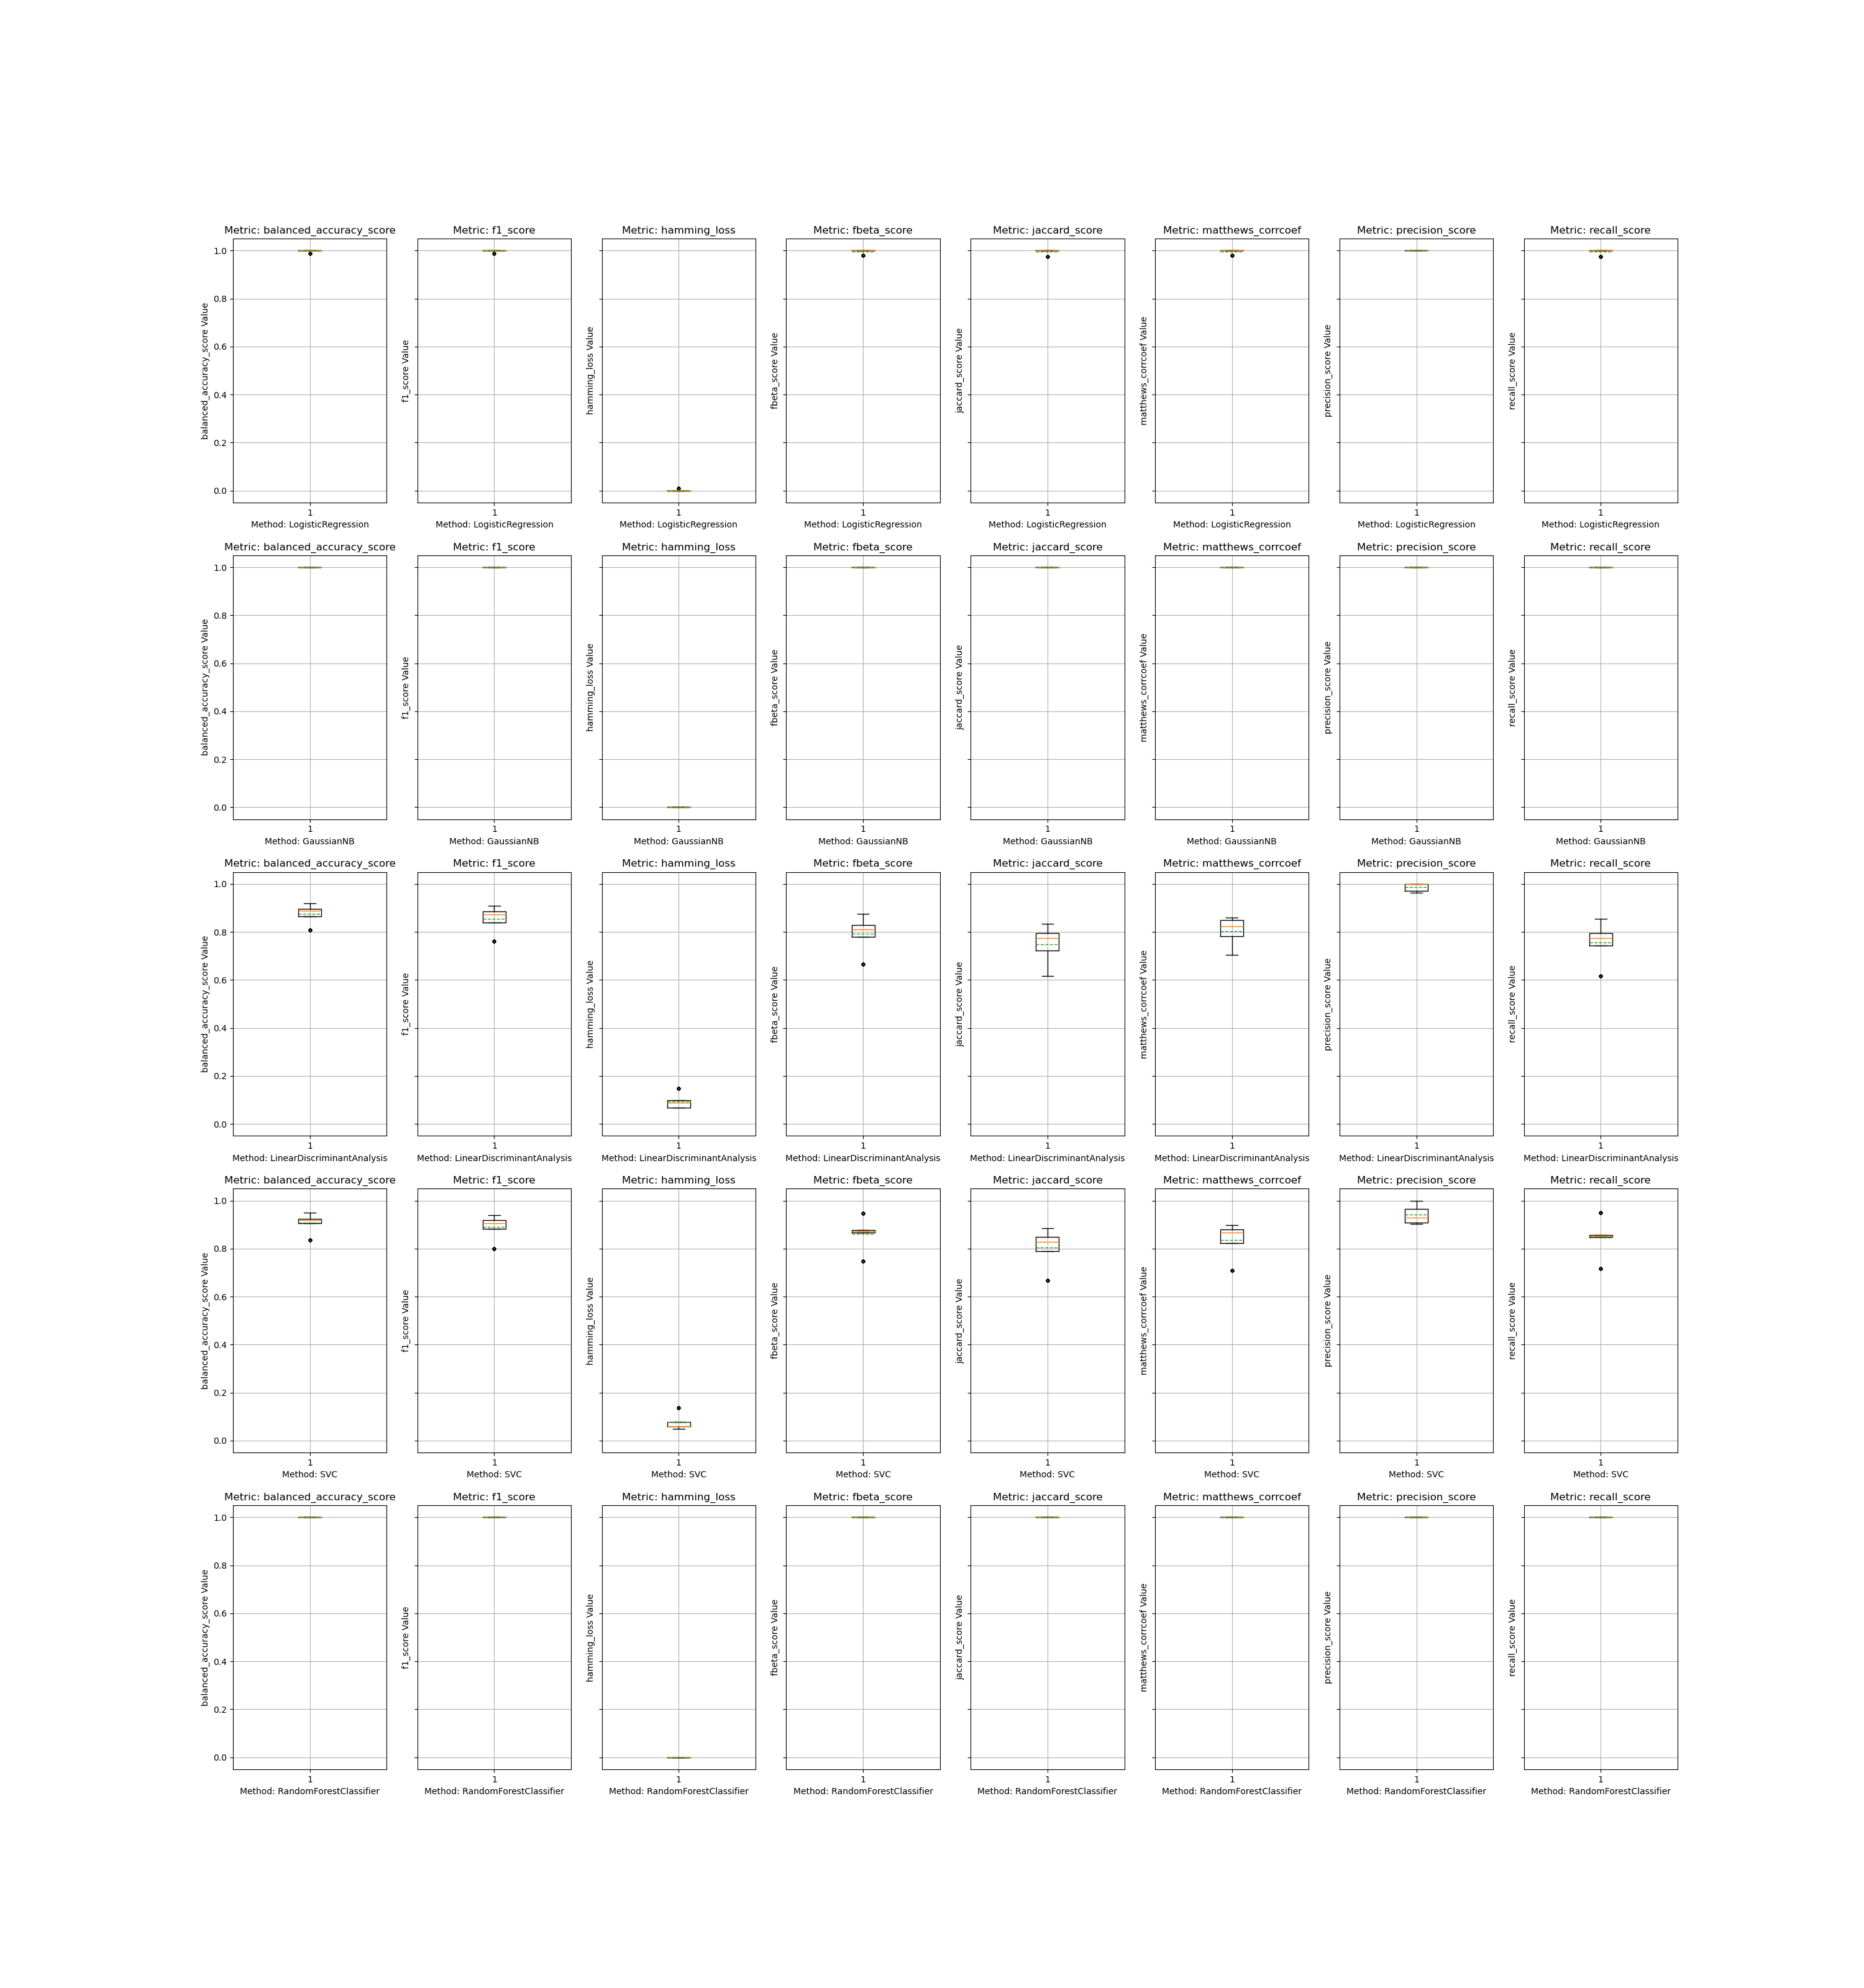
\includegraphics[width=0.95\textwidth]{figures/RNCV/BonusMI/All loop outer folds boxplots.png}
        \caption{Final distributions of all loops of the feature selected model using Mutual Information Select k best}\label{fig:bonusMI}
    \end{center}
\end{figure}

\begin{multicols}{2}

    In comparison to the PCA this feature selection has performed better, the assumption is that since the principled component analysis needs z-scaling before hand and we have not done this that it has performed worse. The Mutual Information infact has metrics that reach 1 which is most likely overfitting than anything else.
    \newline

    \subsection{Optimized} \label{subsec:opted model}

\end{multicols}

\begin{figure}[H]
    \begin{center}
        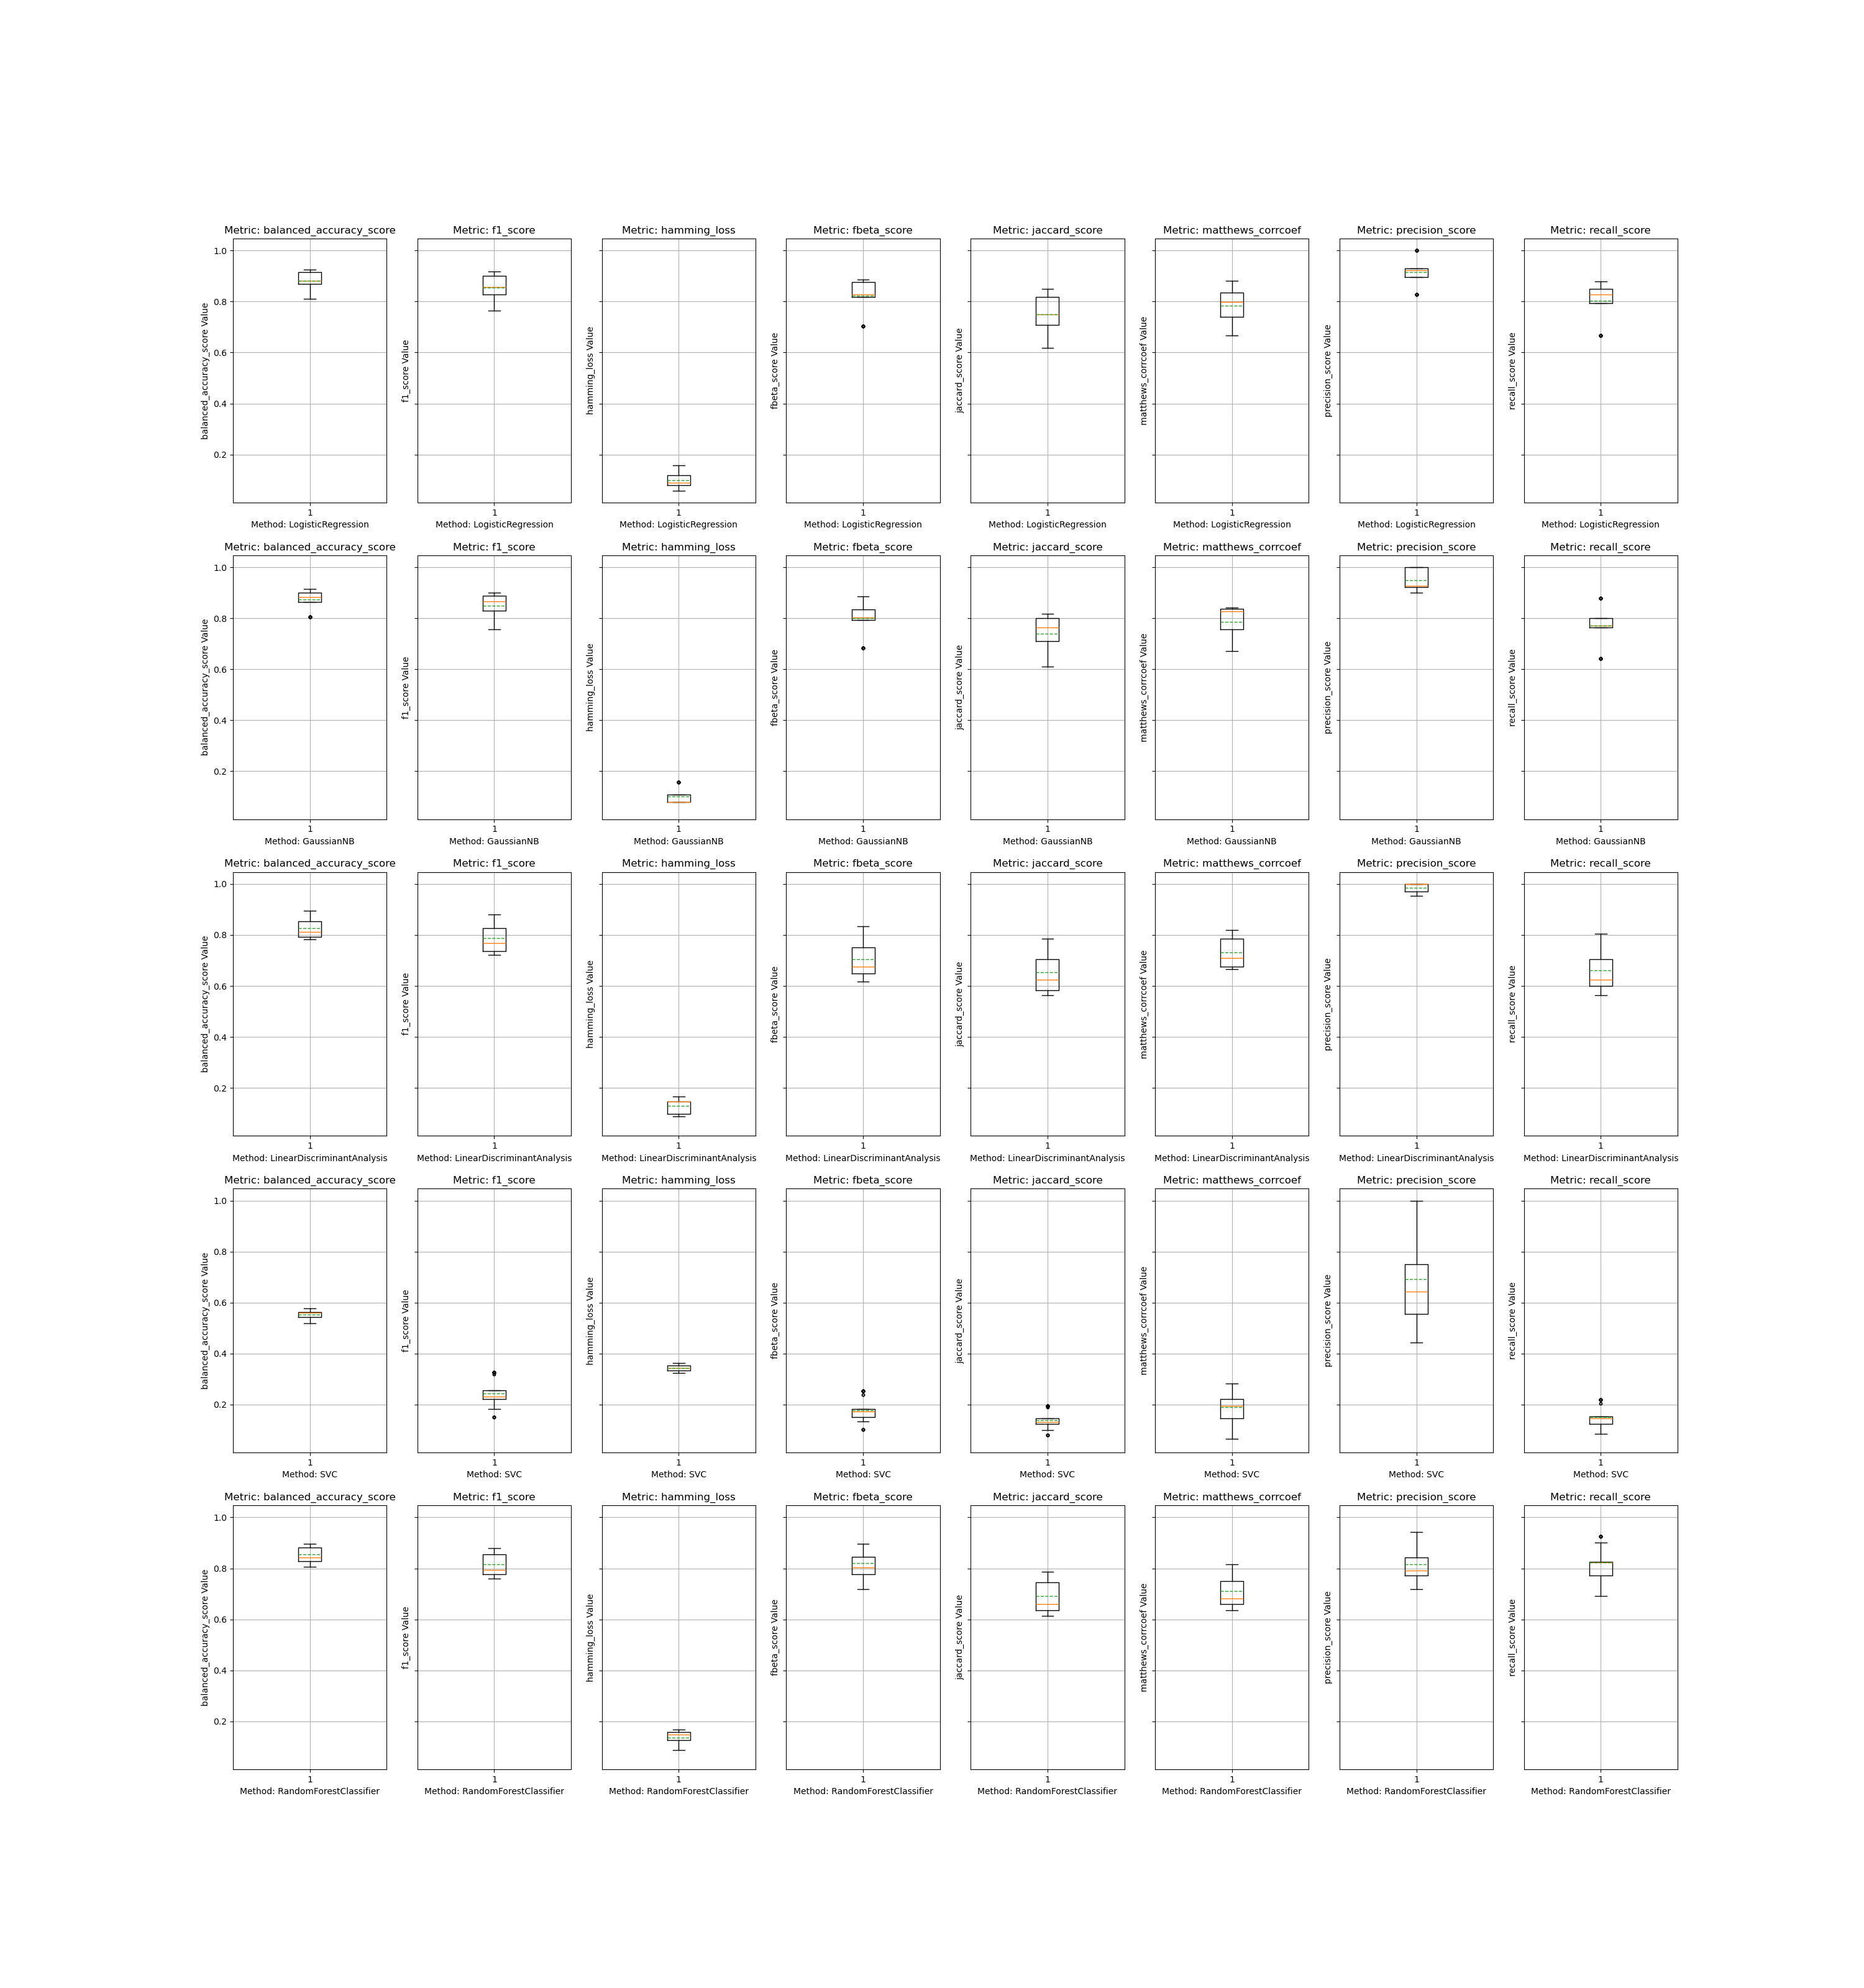
\includegraphics[width=0.95\textwidth]{figures/RNCV/Optimized/All loop outer folds boxplots.png}
        \caption{Final distributions of all loops of the optimized model}\label{fig:optuna desc}
    \end{center}
\end{figure}

\begin{multicols}{2}

    We can see that in our attempt to optimize for the fbeta score some of our models worsen quite alot for all metrics. We can see some marginal improvements on the fbeta score for some of the models (the mean and median value may remain the same but the distribution has leaned higher). The shape of the distributions of most of the models is similar to before. We can be sure that the SVC is not fit for this task. Keeping in mind that this optimized model uses the same feature selection as before we can see many improvements on the fbeta score and some other metrics for some of our models (for instance the Gaussian Naive Bayes and some of the metrics of the Linear Discriminant Analysis).
    \newline

    \section{Conclusions} \label{sec:conc}

    Our best models have to be between the Random Forest classifier, the Gaussian Naive Bayes classifier and the Logistic Regression. We will train our winner on the whole dataset with the optimized parameter of one of these models, the Logistic Regression since it boasts one of the best fbeta scores that we care most for while maintaining very high metrics for the rest of the metrics (or low for the Hamming loss) and in particular the recall score which we care much for. This classification task an be solved well, to a high degree of satisfaction with relatively low amounts of data for the proper classification of both precision and recall.
    \newline

    \section{Disclaimer} \label{sec:disc}

    Large language models (LLM's) were used during the assignment.

    \subsection{LLM} \label{subsec:llms}

    Open AI: Chat GPT 4.0 \cite{noauthor_chatgpt_nodate}

    \subsection{Purpose} \label{subsec:llmUse}

    \begin{enumerate} \label{enm:llm}
        \item To ask if concepts already exist in some dependency.
        \item For acquisition of the relative documentation.
        \item For helping with the \LaTeX table formatting in this report for time efficiency.
        \item Debugging help
        \item In the function "plotKfoldSummary" to help with getting the box plots of all folds into one axis since 5 different box plots in each axis was generated until the .flatten method was called
        \item For help when saving the winner since the models were ran but the winner was not saved so in order to save the winner we had to load back in a model from joblib but new methods had been added to the class. The help was to ask if when we load back in a model the new methods will be brought in, apparently they do since the pkl file keeps the attribute values and re calls the class upon loading from joblib with the parameters so it inherits the new methods.
    \end{enumerate}

    \section{Citations} \label{sec:citations}

    \printbibliography

\end{multicols}

\end{document}

